\begin{frame}
  \frametitle{Literature Review}
  \textbf{Control Rods in MSR}
  \begin{itemize}
    \item MSRs contain comparatively fewer control rods than most other reactor types due to:
      \begin{itemize}
        \item Uniform liquid fuel burnup
        \item Strong passive safety of the liquid fuel form
        \item Low excess reactivity of fuel inventory*
        \item Availability of other control mechanisms:
        \begin{itemize}
          \item Varying pump speeds
          \item Varying heat removal rates at the heat exchangers
          \item Online refueling and salt processing*
        \end{itemize}
      \end{itemize}
    \item Many MSR designs include control rods to facilitate reactor start-up or shut-down rather
      than reactivity control during power operation.
  \end{itemize}
  \pause
  \textbf{Nevertheless, it is important to characterize control rod effects in all relevant
  transient scenarios.}
\end{frame}

\begin{frame}
  \frametitle{Literature Review}
  \textbf{The Control Rod Modeling Dilemma}
  \begin{enumerate}
    \item Neutron diffusion, $P_1$, and $SP_N$ methods perform poorly near control rod regions
      due to the highly anisotropic neutron fluxes and steep flux gradients.
    \item High-fidelity neutron transport methods remain too computationally expensive for routine
      time-dependent multiphysics simulations.
  \end{enumerate}
\end{frame}

\begin{frame}
  \frametitle{Literature Review}
  \textbf{Control Rod Modeling in MSR Multiphysics Studies}

  Common simplifications applied to control rod modeling include:
  \begin{itemize}
    \item Homogenized geometries containing static control rods with albedo neutron flux boundary
      conditions \cite{kophazi_development_2009} or transport-corrected cross sections
      \cite{cui_development_2021, jaradat_development_2021, yang_development_2022}
    \item Scaling the neutron source term to simulate moving control rods
      \cite{delpech_benchmark_2003, krepel_dyn3d-msr_2007, jaradat_development_2021,
      yang_development_2022}
  \end{itemize}

  \begin{block}{\textbf{Technical Gap}}
    \textbf{There are no existing MSR simulation tools or studies involving moving control rods
    which are explicitly modeled.}
  \end{block}
\end{frame}

\begin{frame}
  \frametitle{Literature Review}
  \textbf{Transport-Correction Techniques For Neutron Diffusion-Based Solvers}
  \vspace{.3cm}

  Techniques for augmenting the neutron diffusion method with corrections derived from neutron
  transport
  \begin{itemize}
    \item Absorber Blackness
    \item Method of Equivalent Cross Sections (MECS)
    \item Response-Based Methods
    \item Ronen Method
    \item Transport-Corrected Diffusion Theory
    \item General Equivalence Theory (GET)
    \item Superhomogenization Method (SPH)
  \end{itemize}
\end{frame}

\begin{frame}
  \frametitle{Literature Review}
  \textbf{Absorber Blackness} \\
  Encompasses a broad class of procedures for generating boundary conditions to match approximate
  solutions of low-order methods to more accurate solutions of high-order methods
  \cite{davison_influence_1951, spinks_extrapolation_1965, pellaud_extrapolation_1968,
  mendelson_two-dimensional_1969}. \\
  The boundary conditions are generalizations of the Marshak boundary condition, which in 1-D are
  of the form:
  %
  \begin{align}
    \frac{\phi(x)}{d\phi(x)/dx} =& \lambda \label{eq:marshak}
    \shortintertext{where}
    \phi =& \mbox{ neutron scalar flux,} \nonumber \\
    \lambda =& \mbox{ linear extrapolation length.} \nonumber
  \end{align}
  %
  Alternatively, the internal boundary conditions may be replaced with ``effective'' diffusion
  coefficients and absorption cross sections \cite{bretscher_computing_1997}.
\end{frame}

\begin{frame}
  \frametitle{Literature Review}
  \textbf{Method of Equivalent Cross Sections (MECS)}
  \begin{columns}
    \column[t]{7cm}
    \vspace{.1cm}

    Implemented in the CITATION nodal diffusion code for control rod modeling in High-Temperature
    Gas-Cooled Reactors (HTGR). \\
    \textbf{Methodology}
    \begin{enumerate}
      \item Run a high-fidelity 1-D neutron transport calculation on a representative supercell of
        the control rod and its vicinity
      \item Match the net leakage rates from the transport solver to the diffusion solver using an
        analytic formula
      \item Solve for the equivalent diffusion coefficients
    \end{enumerate}
%    \textbf{Limitations}
%    \begin{enumerate}
%      \item The solving procedure places geometric constraints on the geometry nodalization
%      \item Incompatible with reactor geometries which contain control rods that are too close
%      \item Only applicable for coarse-mesh diffusion solvers
%    \end{enumerate}
    \column[t]{4cm}
    \begin{figure}
      \centering
      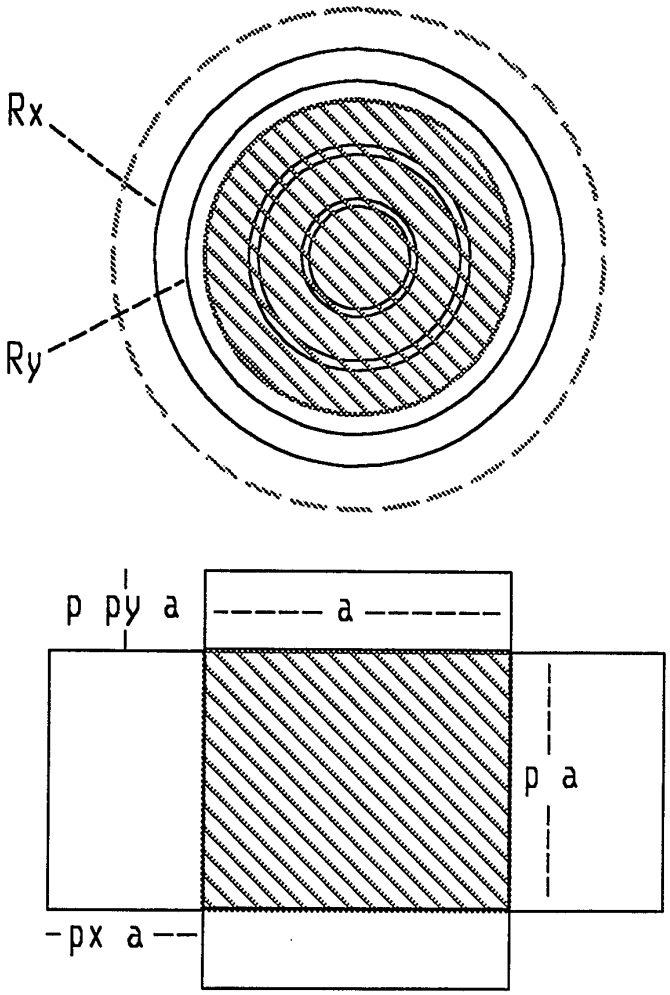
\includegraphics[width=.75\columnwidth]{../images/mecs-geometry}
      \caption{Geometry of the supercell (top) and the diffusion solver mesh (bottom)
        \cite{fen_modelling_1992}.}
    \end{figure}
  \end{columns}
\end{frame}

\begin{frame}
  \frametitle{Literature Review}
  \textbf{Response-Based Methods}
  \vspace{.3cm}

  Another technique applied to modeling control rods in HTGRs with nodal diffusion codes. \\
  Uses neutron transport solutions to generate response functions, which relate flux-based
  quantities (e.g., incident partial currents $\Rightarrow$ average nodal flux and outgoing partial
  currents)
  \vspace{.3cm}

  \textbf{Examples}
  \begin{enumerate}
    \item Fen et al. \cite{fen_modelling_1992} developed the Response Matrix Method which generates
      boundary conditions from response functions.
    \item Rahnema et al. \cite{rahnema_advanced_2011} developed the integrated diffusion/transport
      (IDT) method which generates coupling coefficients used in nodal diffusion calculations.
  \end{enumerate}
\end{frame}

\begin{frame}
  \frametitle{Literature Review}
  \textbf{The Ronen Method} \\
  Ronen \cite{ronen_accurate_2004} derived transport operators representing accurate, analytical
  relations between neutron current and neutron flux. \\
  Starting with an initial neutron diffusion
  flux solution, the operators are used to iteratively improve the flux solution by updating the
  diffusion coefficients as follows:
  %
  \begin{align}
    D(\vec{r},E) =& -\frac{J_{tr}(\vec{r},E)}{\nabla \phi(\vec{r},E)}
    \label{eq:ronen}
    \shortintertext{where}
    J_{tr} =& \mbox{ transport-derived neutron current.} \nonumber
  \end{align}
  %
  Ronen derived transport operators from the integral transport equations for a 1-D homogeneous
  region with two groups and isotropic scattering. \\
  Others numerically implemented the Ronen method \cite{tomatis_application_2011} and extended the
  method for 1-D heterogeneous geometries \cite{gross_high-accuracy_2020} and incorporated
  acceleration schemes \cite{tomatis_ronen_2021}.
\end{frame}

\begin{frame}
  \frametitle{Literature Review}
  \textbf{Transport-Corrected Diffusion Theory}
  \vspace{.2cm}

  Pounders \& Rahnema \cite{pounders_diffusion_2009} developed two separate methods which also
  generate space-dependent diffusion coefficients for transport corrections. \\
  Both methods require a priori knowledge of the neutron flux and current.
  \vspace{.2cm}
  \begin{columns}
    \column[t]{.5\textwidth}
    \textbf{1) Averaged Eddington Factor Diffusion Theory}
    %
    \begin{align}
      \small
      E_g(z) =& \frac{\int^1_{-1} \mu^2\psi(z,\mu)d\mu}{\int^1_{-1} \psi(z,\mu)d\mu}
    \end{align}
    %
    \begin{align}
      \small
      D^{AEF}_g(z) =& E^i_g\left[\hat{\Sigma}_{t,g}-\sum^G_{g'=1}\hat{\Sigma}^{g'\rightarrow g}_{s1}
      \frac{\hat{J}_{g'}}{\hat{J}_g}\right]^{-1}
    \end{align}
    \hfill
    \column[t]{.5\textwidth}
    \textbf{2) High-Order Empirical Diffusion Coefficients}
    \begin{align}
      D^i_g =& -\frac{\left(z_{i+1}-z_i\right) \bar{J}_g}{\left[\phi_g(z_{i+1})-\phi_g(z_i)\right]}
      \label{eq:emp}
    \end{align}
  \end{columns}
\end{frame}

\begin{frame}
  \frametitle{Literature Review}
  \begin{block}{\textbf{Summary}}
    \begin{itemize}
      \item Neutron diffusion methods fare poorly near control rod regions, but neutron transport
        methods are too computationally expensive for routine time-dependent multiphysics simulations
      \item Various transport-correction techniques exist for neutron diffusion-based solvers
      \item Equivalence techniques are popular and perform well in many use cases. However,
        \begin{itemize}
          \item Equivalent cross sections cannot capture anisotropic effects
          \item Equivalent boundary conditions/discontinuity factors are complicated to define for
            irregular geometries
        \end{itemize}
      \item Demonstrations of the Ronen method are limited to 1-D geometries due to the difficulty of
        deriving transport operators for complex 2-D and 3-D geometries
      \item The transport-corrected diffusion theories by Pounders \& Rahnema require a priori
        knowledge of the neutron flux and current
    \end{itemize}
  \end{block}
\end{frame}
